\documentclass[10pt]{article}
\usepackage[polish]{babel}
\usepackage[utf8]{inputenc}
\usepackage[T1]{fontenc}
\usepackage{amsmath}
\usepackage{amsfonts}
\usepackage{amssymb}
\usepackage[version=4]{mhchem}
\usepackage{stmaryrd}
\usepackage{graphicx}
\usepackage[export]{adjustbox}
\graphicspath{ {./images/} }

\title{EGZAMIN WSTĘPNY Z MATEMATYKI }

\author{}
\date{}


\begin{document}
\maketitle
Egzamin składa się z 30 zadań. Zadania 1-10 oceniane będą w skali 0-2 punkty, zadania \(11-30\) w skali \(0-4\) punkty. Czas trwania egzaminu - 240 minut.

\section*{Powodzenia!}
\begin{enumerate}
  \item Znaleźć wszystkie rozwiązania równania \(81 x^{4}-72 x^{2}=-16\).
  \item Zbiory \(A, B\) i \(A \cup B\) mają odpowiednio 1999, 2049 i 3998 elementów. Ile elementów mają odpowiednio zbiory \(A-B\) i \(A \cap B\) ?
  \item Jeden metr ma 1000000 mikronów, a 100000000 angstremów to jeden centymetr. Ile angstremów ma jeden mikron?
  \item Rozwiązać równanie \(\log _{2}(-2)^{5 n}=n^{2}+4\), w którym \(n\) jest liczbą naturalną.
  \item Obliczyć \(\binom{n}{5}\), jeśli wiadomo, że \(\binom{n}{3}=\binom{n}{4}\).
  \item Rozwiązać nierówność \(|x-1| \leqslant \frac{x}{3}+1\).
  \item Dana jest funkcja \(f(x)=(x-1)^{2}\). Na osobnych rysunkach naszkicować wykresy funkcji: (a) \(y=f(x)\) ;(b) \(y=f(-x)\) ;(c) \(y=f(x+1)-2\).
  \item Rozwiązać nierówność \(x+3 \leqslant \frac{10}{x}\).
  \item Dla jakich wartości \(x\) istnieje trójkąt o bokach długości \(1,2, \log x\) ?
  \item W trójkącie naprzeciw boku długości \(3 \sqrt{2}\) leży kąt miary \(45^{\circ}\). Wyznaczyć promień okręgu opisanego na tym trójkącie.
  \item Mamy dwa naczynia, z których jedno zawiera 10 litrów wody, a drugie 10 litrów soku. Połowę wody przelewamy do soku, mieszamy, a następnie połowę roztworu przelewamy z powrotem do wody. Obliczyć procentowe stężenia otrzymanych roztworów.
  \item Punkty \(A(-1,0), B(3,2)\) i \(C(5,-2)\) są wierzchołkami trójkąta. Pokazać, że jest to trójkąt równoramienny. Napisać równanie osi symetrii tego trójkąta.
  \item Doprowadzić do najprostszej postaci wyrażenie \(\frac{x+2+\sqrt{x^{2}-4}}{x+2-\sqrt{x^{2}-4}}+\frac{x+2-\sqrt{x^{2}-4}}{x+2+\sqrt{x^{2}-4}}\).
  \item W obszar między trzema wzajemnie stycznymi okręgami o promieniu \(R\) wpisano okrąg. Znaleźć promień \(r\) tego okręgu.
  \item Funkcję \(f(x)=x^{5}-9 x^{3}-27 x^{2}+243\) zapisać w postaci iloczynowej i następnie rozwiązać nierówność \(f(x)>0\).
  \item Pokazać, że funkcja \(f(x)=x^{2}\) ma minimum lokalne w punkcie \(x_{0}=0\). Uzasadnić, że funkcja \(g(x)=\left\{\begin{array}{r}x^{2} \text { dla } x \neq 0 \\ 1 \text { dla } x=0\end{array}\right.\) ma maksi-\\
mum lokalne w punkcie \(x_{0}=0\), zob. rys. 1.
  \item Napisać równania tych stycznych do wykresu funkcji \(y=\frac{x^{2}}{x-2}\), które są równoległe\\
mum lokalne w punkcie \(x_{0}=0\), zob. rys. 1.
  \item Napisać równania tych stycznych do wykresu funkcji \(y=\frac{x^{2}}{x-2}\), które są równoległe\\
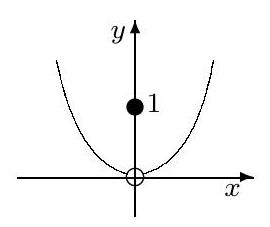
\includegraphics[max width=\textwidth, center]{2024_11_21_80c827237e5b1a9f7989g-2(1)}\\
do prostej \(3 x+y=0\).
  \item Wyznaczyć największą i najmniejszą wartość funkcji \(f(x)=x+\sqrt{1-x^{2}}\).
  \item Znaleźć asymptoty wykresu funkcji \(y=\frac{4 x^{2}+9 x}{x-4}\).
  \item Rozwiązać równanie \(3^{2 x}-2 \cdot 3^{x}+a=0\), w którym \(a=\lim _{n \rightarrow \infty} \frac{\sqrt{n^{2}+3}-4 n}{n-1}\).
  \item W prostokątnym układzie współrzędnych zaznaczyć zbiór punktów \((x, y)\), których współrzędne spełniają równanie \(\log _{2}(x+y)=\log _{2} x+\log _{2} y\).
  \item Obliczyć średnią arytmetyczną tych spośród liczb naturalnych 1, 2, 3, .., 2000, które nie są podzielne przez 5.
  \item Wyznaczyć ciąg geometryczny \(a_{1}, a_{2}, \ldots, a_{n}, \ldots\), jeżeli wiadomo, że \(a_{1}+a_{2}+a_{3}+a_{4}=30\) i \(a_{2}+a_{3}+a_{4}+a_{5}=60\). Znaleźć taką liczbę \(n\), że \(a_{n}<500000<a_{n+1}\).
  \item Rozwiązać równanie \(2 \sin ^{2} x+\sin 2 x=2\).
  \item Rozwiązać nierówność \(\sin ^{2} x>\frac{3}{4}\) dla \(x \in\langle 0 ; 2 \pi\rangle\).
  \item Znaleźć równania prostych przechodzących przez punkt \(A(7,3)\) i przecinających prostą \(x-3 y-1=0\) pod kątem \(45^{\circ}\).
  \item Obliczyć długość najkrótszej drogi poprowadzonej po powierzchni sześcianu o krawędziach długości 1 i łączącej dwa przeciwległe wierzchołki tego sześcianu. Ile najkrótszych dróg łączy dwa wybrane przeciwległe wierzchołki tego sześcianu?
  \item Obliczyć iloczyn skalarny wektorów \(\vec{a}=[-1,1+x]\) i \(\vec{b}=[\sqrt{x+3}, 1]\). Dla jakich \(x\) wektory \(\vec{a}\) i \(\vec{b}\) są prostopadłe? Jaki kąt (ostry, prosty, czy rozwarty) tworzą te wektory dla \(x=-2\) ?
  \item Rzucono pięć razy dwiema kostkami do gry. Obliczyć prawdopodobieństwo tego, że co najmniej dwa razy suma oczek na obu kostkach jest nie mniejsza od 10.
  \item Sześcian o krawędzi długości \(a\) podzielono płaszczyzną przechodzacą przez przekątną jednej z jego ścian i przez środki dwóch krawędzi leżących na przeciwległej ścianie na dwie bryły, zob. rys. 2. Obliczyć objętości obu otrzymanych brył.\\
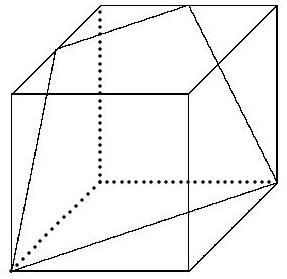
\includegraphics[max width=\textwidth, center]{2024_11_21_80c827237e5b1a9f7989g-2}
\end{enumerate}

Rys. 2


\end{document}